\documentclass[letterpaper]{article}
%\documentclass[a5paper]{article}

%% Language and font encodings
\usepackage[english]{babel}
\usepackage[utf8x]{inputenc}
\usepackage[T1]{fontenc}

%% Sets page size and margins
\usepackage[letterpaper,top=.75in,bottom=1in,left=1in,right=1in,marginparwidth=1.75cm]{geometry}
%\usepackage[a5paper,top=1cm,bottom=1cm,left=1cm,right=1.5cm,marginparwidth=1.75cm]{geometry}

\usepackage{graphicx}
%\graphicspath{../images}	  %%where to look for images

%% Useful packages
\usepackage{amssymb, amsmath, amsthm} 
%\usepackage{graphicx}  %%this is currently enabled in the default document, so it is commented out here. 
\usepackage{calrsfs}
\usepackage{braket}
\usepackage{mathtools}
\usepackage{lipsum}
\usepackage{tikz}
\usetikzlibrary{cd}
\usepackage{verbatim}
%\usepackage{ntheorem}% for theorem-like environments
\usepackage{mdframed}%can make highlighted boxes of text
%Use case: https://tex.stackexchange.com/questions/46828/how-to-highlight-important-parts-with-a-gray-background
\usepackage{wrapfig}
\usepackage{centernot}
\usepackage{subcaption}%\begin{subfigure}{0.5\textwidth}
\usepackage{pgfplots}
\pgfplotsset{compat=1.13}
\usepackage[colorinlistoftodos]{todonotes}
\usepackage[colorlinks=true, allcolors=blue]{hyperref}
\usepackage{xfrac}					%to make slanted fractions \sfrac{numerator}{denominator}
\usepackage{enumitem}            
    %syntax: \begin{enumerate}[label=(\alph*)]
    %possible arguments: f \alph*, \Alph*, \arabic*, \roman* and \Roman*
\usetikzlibrary{arrows,shapes.geometric,fit}

\DeclareMathAlphabet{\pazocal}{OMS}{zplm}{m}{n}
%% Use \pazocal{letter} to typeset a letter in the other kind 
%%  of math calligraphic font. 

%% This puts the QED block at the end of each proof, the way I like it. 
\renewenvironment{proof}{{\bfseries Proof}}{\qed}
\makeatletter
\renewenvironment{proof}[1][\bfseries \proofname]{\par
  \pushQED{\qed}%
  \normalfont \topsep6\p@\@plus6\p@\relax
  \trivlist
  %\itemindent\normalparindent
  \item[\hskip\labelsep
        \scshape
    #1\@addpunct{}]\ignorespaces
}{%
  \popQED\endtrivlist\@endpefalse
}
\makeatother

%% This adds a \rewnewtheorem command, which enables me to override the settings for theorems contained in this document.
\makeatletter
\def\renewtheorem#1{%
  \expandafter\let\csname#1\endcsname\relax
  \expandafter\let\csname c@#1\endcsname\relax
  \gdef\renewtheorem@envname{#1}
  \renewtheorem@secpar
}
\def\renewtheorem@secpar{\@ifnextchar[{\renewtheorem@numberedlike}{\renewtheorem@nonumberedlike}}
\def\renewtheorem@numberedlike[#1]#2{\newtheorem{\renewtheorem@envname}[#1]{#2}}
\def\renewtheorem@nonumberedlike#1{  
\def\renewtheorem@caption{#1}
\edef\renewtheorem@nowithin{\noexpand\newtheorem{\renewtheorem@envname}{\renewtheorem@caption}}
\renewtheorem@thirdpar
}
\def\renewtheorem@thirdpar{\@ifnextchar[{\renewtheorem@within}{\renewtheorem@nowithin}}
\def\renewtheorem@within[#1]{\renewtheorem@nowithin[#1]}
\makeatother

%% This makes theorems and definitions with names show up in bold, the way I like it. 
\makeatletter
\def\th@plain{%
  \thm@notefont{}% same as heading font
  \itshape % body font
}
\def\th@definition{%
  \thm@notefont{}% same as heading font
  \normalfont % body font
}
\makeatother

%===============================================
%==============Shortcut Commands================
%===============================================
\newcommand{\ds}{\displaystyle}
\newcommand{\B}{\mathcal{B}}
\newcommand{\C}{\mathbb{C}}
\newcommand{\F}{\mathbb{F}}
\newcommand{\N}{\mathbb{N}}
\newcommand{\R}{\mathbb{R}}
\newcommand{\Q}{\mathbb{Q}}
\newcommand{\T}{\mathcal{T}}
\newcommand{\Z}{\mathbb{Z}}
\renewcommand\qedsymbol{$\blacksquare$}
\newcommand{\qedwhite}{\hfill\ensuremath{\square}}
\newcommand*\conj[1]{\overline{#1}}
\newcommand*\closure[1]{\overline{#1}}
\newcommand*\mean[1]{\overline{#1}}
%\newcommand{\inner}[1]{\left< #1 \right>}
\newcommand{\inner}[2]{\left< #1, #2 \right>}
\newcommand{\powerset}[1]{\pazocal{P}(#1)}
%% Use \pazocal{letter} to typeset a letter in the other kind 
%%  of math calligraphic font. 
\newcommand{\cardinality}[1]{\left| #1 \right|}
\newcommand{\domain}[1]{\mathcal{D}(#1)}
\newcommand{\image}{\text{Im}}
\newcommand{\inv}[1]{#1^{-1}}
\newcommand{\preimage}[2]{#1^{-1}\left(#2\right)}
\newcommand{\script}[1]{\mathcal{#1}}


\newenvironment{highlight}{\begin{mdframed}[backgroundcolor=gray!20]}{\end{mdframed}}

\DeclarePairedDelimiter\ceil{\lceil}{\rceil}
\DeclarePairedDelimiter\floor{\lfloor}{\rfloor}

%===============================================
%===============My Tikz Commands================
%===============================================
\newcommand{\drawsquiggle}[1]{\draw[shift={(#1,0)}] (.005,.05) -- (-.005,.02) -- (.005,-.02) -- (-.005,-.05);}
\newcommand{\drawpoint}[2]{\draw[*-*] (#1,0.01) node[below, shift={(0,-.2)}] {#2};}
\newcommand{\drawopoint}[2]{\draw[o-o] (#1,0.01) node[below, shift={(0,-.2)}] {#2};}
\newcommand{\drawlpoint}[2]{\draw (#1,0.02) -- (#1,-0.02) node[below] {#2};}
\newcommand{\drawlbrack}[2]{\draw (#1+.01,0.02) --(#1,0.02) -- (#1,-0.02) -- (#1+.01,-0.02) node[below, shift={(-.01,0)}] {#2};}
\newcommand{\drawrbrack}[2]{\draw (#1-.01,0.02) --(#1,0.02) -- (#1,-0.02) -- (#1-.01,-0.02) node[below, shift={(+.01,0)}] {#2};}

%***********************************************
%**************Start of Document****************
%***********************************************

%===============================================
%===============Theorem Styles==================
%===============================================

%================Default Style==================
\theoremstyle{plain}% is the default. it sets the text in italic and adds extra space above and below the \newtheorems listed below it in the input. it is recommended for theorems, corollaries, lemmas, propositions, conjectures, criteria, and (possibly; depends on the subject area) algorithms.
\newtheorem{theorem}{Theorem}
\numberwithin{theorem}{section} %This sets the numbering system for theorems to number them down to the {argument} level. I have it set to number down to the {section} level right now.
\newtheorem*{theorem*}{Theorem} %Theorem with no numbering
\newtheorem{corollary}[theorem]{Corollary}
\newtheorem*{corollary*}{Corollary}
\newtheorem{conjecture}[theorem]{Conjecture}
\newtheorem{lemma}[theorem]{Lemma}
\newtheorem*{lemma*}{Lemma}
\newtheorem{proposition}[theorem]{Proposition}
\newtheorem*{proposition*}{Proposition}
\newtheorem{problemstatement}[theorem]{Problem Statement}


%==============Definition Style=================
\theoremstyle{definition}% adds extra space above and below, but sets the text in roman. it is recommended for definitions, conditions, problems, and examples; i've alse seen it used for exercises.
\newtheorem{definition}[theorem]{Definition}
\newtheorem*{definition*}{Definition}
\newtheorem{condition}[theorem]{Condition}
\newtheorem{problem}[theorem]{Problem}
\newtheorem{example}[theorem]{Example}
\newtheorem*{example*}{Example}
\newtheorem*{counterexample*}{Counterexample}
\newtheorem*{romantheorem*}{Theorem} %Theorem with no numbering
\newtheorem{exercise}{Exercise}
\numberwithin{exercise}{section}
\newtheorem{algorithm}[theorem]{Algorithm}

%================Remark Style===================
\theoremstyle{remark}% is set in roman, with no additional space above or below. it is recommended for remarks, notes, notation, claims, summaries, acknowledgments, cases, and conclusions.
\newtheorem{remark}[theorem]{Remark}
\newtheorem*{remark*}{Remark}
\newtheorem{notation}[theorem]{Notation}
\newtheorem*{notation*}{Notation}
%\newtheorem{claim}[theorem]{Claim}  %%use this if you ever want claims to be numbered
\newtheorem*{claim}{Claim}



\pgfplotsset{compat=1.13}

%\newcommand{\T}{\mathcal{T}}
%\newcommand{\B}{\mathcal{B}}
\newcommand{\arbcup}[1]{\bigcup\limits_{\alpha\in\Gamma}#1_\alpha}
\newcommand{\arbcap}[1]{\bigcap\limits_{\alpha\in\Gamma}#1_\alpha}
\newcommand{\arbcoll}[1]{\{#1_\alpha\}_{\alpha\in\Gamma}}
\newcommand{\arbprod}[1]{\prod\limits_{\alpha\in\Gamma}#1_\alpha}

\title{Math 501 \linebreak
Homework 12}
\author{Trevor Klar}

\begin{document}

\maketitle

\begin{enumerate}
\item Let $X$ be a topological space, with $\B$ a basis for the topology on $X$. Prove that if every open cover of $X$ by sets in $\B$ has a finite subcover, then $X$ is compact. 
\begin{proof}
Let $\arbcoll{U}$ be an arbitrary open cover of $X$. Since each $U_\alpha$ is open, we know that for each $x\in U_\alpha$, there exists a basic open set $B$ such that $x\in B \subset U_\alpha$. So for each $\alpha\in\Gamma$, and each $x\in U_\alpha$, let $B_{(\alpha,x)}$ denote a basic open set such that $x\in B \subset U_\alpha$. This means that $\bigcup_{\alpha\in\Gamma}\{B_{(\alpha,x)} : \forall x\in U_\alpha \}$ is an open cover of $X$ by sets in $\B$, so it has a finite subcover $\{B_i\}_{i=1}^N$. Each $B_i$ is a subset of some $U_\alpha$, so for each $i\in\{1, \ldots, N\}$, let $\alpha_i$ be an element of $\Gamma$ such that $B_i\subset U_{\alpha_i}$. Therefore, $\bigcup_{i=1}^N \{\{U_{\alpha_i}\}\}$ is a finite subcollection of $\arbcoll{U}$ which covers $X$, so $X$ is compact.\footnote{There could be $U_{\alpha_i}=U_{\alpha_j}$ for some $i\neq j$, so this union notation is used to to clarify the fact that this is a collection of sets which does not repeat. It is a union of singletons of sets, not a union of the sets themselves.} 
\end{proof}

\item Let $\arbcoll{X}$ be a collection of spaces. 

	\begin{enumerate}
	\item Prove that the projection $\pi_\beta:\arbprod{X}\to X_\beta$ is not necessarily closed. 
	\begin{proof}
	Consider the graph of $\tan|_{(-\frac{\pi}{2},\frac{\pi}{2})}$ as a subset of $\R^2_{usual}$; $S=\{(x,tan(x) : -\frac{\pi}{2}<x<\frac{\pi}{2}\}$. 
	
	\begin{center}
	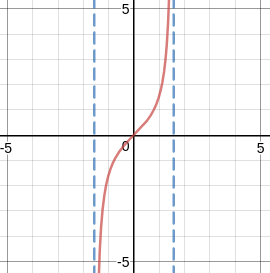
\includegraphics[scale=.3]{hw12_prob2a}
	\end{center}
	
	This set $S$ is closed in $\R^2$, but $\pi_1(S)=(-\frac{\pi}{2},\frac{\pi}{2})$ is not closed in $\R$. 
	\end{proof}
	
	\item Prove that $g:Y\to \arbprod{X}$ is continuous if and only if $\pi_\alpha\circ g$ is continuous for each $\alpha\in\Gamma$. 
	\begin{proof}[\textbf{Proof ($\implies$)}]
	Suppose $g:Y\to \arbprod{X}$ is continuous. To show that $\pi_\alpha \circ g : Y \to X_{\alpha}$ is continuous for each $\alpha\in\Gamma$; let $\beta\in\Gamma$ be arbitrary, and let $U_\beta$ be an arbitrary open set in $X_\beta$. Now, 
	$$\preimage{\pi_\beta}{U_\beta}=U_\beta \times \prod\limits_{\alpha\in(\Gamma-\beta)}{X_\alpha}_,$$
	Which is open in $\arbprod{X}$. Since $g$ is continuous, then $\preimage{g}{\preimage{\pi_\beta}{U_\beta}} = \preimage{(\pi_\alpha\circ g)}{U_\beta}$ is open in $Y$, and we are done. 
	\end{proof}
	\begin{proof}[\textbf{Proof ($\impliedby$)}]
	Suppose that $\pi_\alpha \circ g : Y \to X_{\alpha}$ is continuous for each $\alpha\in\Gamma$. Let $U\in\arbprod{X}$ be any basic open set. By definition, 
	\[
	U = \prod	
	\begin{cases}
	U_\alpha & \alpha\in \{\alpha_1, \ldots, \alpha_N\}\\
	X_\alpha & \alpha\not\in \{\alpha_1, \ldots, \alpha_N\}\\
	\end{cases}
	\]
	
	
	
	 Now we can see that $\preimage{g}{U}$ is open by the following diagram chase, since there are finitely many nontrivial component sets of $U$:
	
	\[
	\begin{tikzcd}
	Y \arrow[r, "g"] \arrow[rr, bend left, "\pi_\alpha \circ g"]& \arbprod{X} \arrow[r, "\pi_\alpha"]  & X_\alpha
	\end{tikzcd}
	\]
	
	For each $\alpha_i\in \{\alpha_1, \ldots, \alpha_N\}$, denote the preimage 
	$$\preimage{(\pi_{\alpha_i} \circ g)}{U_{\alpha_i}} = {V_{\alpha_i}}.$$ 
	Note that $V_{\alpha_i}$ may differ from $g^{-1}(U)$, since $\preimage{\pi_{\alpha_i}}{\pi_{\alpha_i}(U)}$ may differ from $U$. However, $g^{-1}(U) \subset V_{\alpha_i}$. We know that $V_{\alpha_i}$ is open, since $\pi_{\alpha_i} \circ g$ is continuous. Now we are done, since $\bigcap V_{\alpha_i} = g^{-1}(U)$ is a finite intersection of open sets, and thus is open. To see that this equality holds, let $p\in\bigcap V_{\alpha_i}$. So, for every $\alpha\in\Gamma$, 
	\[(\pi_{\alpha} \circ g)(p) \in 
	\begin{cases}
	U_\alpha & \alpha\in \{\alpha_1, \ldots, \alpha_N\}\\
	X_\alpha & \alpha\not\in \{\alpha_1, \ldots, \alpha_N\}\\
	\end{cases}
	\]
	
	so $g(p)\in U$. Thus, $\bigcap V_{\alpha_i} \subset g^{-1}(U)$. Now we show that $\bigcap V_{\alpha_i} \supset g^{-1}(U)$. Let $p\in\preimage{g}{U}$. So $g(p)\in U$, and 
	\[(\pi_{\alpha} \circ g)(p) \in 
	\begin{cases}
	U_\alpha & \alpha\in \{\alpha_1, \ldots, \alpha_N\}\\
	X_\alpha & \alpha\not\in \{\alpha_1, \ldots, \alpha_N\}\\
	\end{cases}
	\]
	thus, $p\in\bigcap V_{\alpha_i}$ by definition of $V_{\alpha_i}$. Thus, we have shown that for every basic open set $U$, $\preimage{g}{U}$ is open, therefore $g$ is continuous. 
	\end{proof}
	\end{enumerate}

\item Describe the box topology on $\prod\limits_{x\in X}\{0,1\}_X$. Show that the box topology on $\prod\limits_{x\in X}\{0,1\}_X$ is not necessarily compact. 

\textbf{Answer:} The space itself is the set of all functions $f:X\to\{0,1\}$ such that for all $x\in X$, $f(x)=0$ or $f(x)=1$. The topology is the discrete topology, since a set $U$ is open in $\prod\limits_{x\in X}\{0,1\}_X$ if $\pi_x(U)$ is open for all $x\in X$, and each $\{0,1\}$ has the discrete topology. 

\begin{proof}
To show that the box topology on $\prod\limits_{x\in X}\{0,1\}_X$ is not necessarily compact, consider $\{0,1\}^\N$ where $\N=\{1, 2, \ldots\}$. For each $i\in\N$, let $S_i = \{f:\N\to \{0,1\} | f(i)=1\}$, and let $S_{0}$ be the singleton set $\{f\equiv 0\}$. \\
Now $\{S_i\}_{i=0}^{\infty}$ is an open cover of $\{0,1\}^\N$, since if $f\not\equiv0$ then there is some $i\in\N$ such that $f(i)=1$. Also, this open cover has no finite subcover, since removing any element $S_j$ of the cover results in a collection which does not contain $f:\N\to \{0,1\}$ such that $f(j)=1$ and $f(i)=0$ for all $i\neq j$. 
\end{proof}


\setcounter{enumi}{4}
\item Prove the converse to the Tychonoff Theorem: If the product topology $\arbprod{X}$ is compact, then each $X_\alpha$ is compact. 
\begin{proof}
Suppose $X=\arbprod{X}$ is compact. Let $\alpha_0\in\Gamma$ be arbitrary, and let $\{U_{\beta_{\alpha_0}}\}_{\beta\in\Delta}$ be an arbitrary open cover of $X{\alpha_0}$. Let
$$\{U_\beta\}_{\beta\in\Delta}=\left\lbrace U_{\beta_{\alpha_0}}\times\prod\limits_{\alpha}U_{\beta_\alpha} : \beta\in\Delta, \, \alpha\in(\Gamma-\alpha_0)\right\rbrace$$ 
be an arbitrary open cover of $X$. Since $X$ is compact, $\{U_\beta\}$ has a finite subcover 
$$\{U_{\beta^i}\}_{i=1}^N = \left\lbrace\prod\limits_{\alpha\in\Gamma}U_{\beta^i_\alpha}\right\rbrace_{i=1}^N$$ 
where each $\beta^i\in\Delta$. Now consider the image of this collection in the projection $\pi_{\alpha_0}$:
$$\{\pi_{\alpha_0}\left(U_{\beta^i}\right)\}_{i=1}^N = \{ U_{\beta^i_{\alpha_0}}\}_{i=1}^N$$
Observe that $\{ U_{\beta^i_{\alpha_0}}\}_{i=1}^N \subset \{U_{\beta_{\alpha_0}}\}_{\beta\in\Delta}$, and it also covers all of $X_{\alpha_0}$ (since $\{U_{\beta^i}\}_{i=1}^N$ covers $X$). Thus, we have produced a finite subcover of any open cover of any $X_\alpha$, so we are done. 
\end{proof}

\end{enumerate}

\end{document}
